% Options for packages loaded elsewhere
\PassOptionsToPackage{unicode}{hyperref}
\PassOptionsToPackage{hyphens}{url}
%
\documentclass[
]{book}
\usepackage{lmodern}
\usepackage{amsmath}
\usepackage{ifxetex,ifluatex}
\ifnum 0\ifxetex 1\fi\ifluatex 1\fi=0 % if pdftex
  \usepackage[T1]{fontenc}
  \usepackage[utf8]{inputenc}
  \usepackage{textcomp} % provide euro and other symbols
  \usepackage{amssymb}
\else % if luatex or xetex
  \usepackage{unicode-math}
  \defaultfontfeatures{Scale=MatchLowercase}
  \defaultfontfeatures[\rmfamily]{Ligatures=TeX,Scale=1}
\fi
% Use upquote if available, for straight quotes in verbatim environments
\IfFileExists{upquote.sty}{\usepackage{upquote}}{}
\IfFileExists{microtype.sty}{% use microtype if available
  \usepackage[]{microtype}
  \UseMicrotypeSet[protrusion]{basicmath} % disable protrusion for tt fonts
}{}
\makeatletter
\@ifundefined{KOMAClassName}{% if non-KOMA class
  \IfFileExists{parskip.sty}{%
    \usepackage{parskip}
  }{% else
    \setlength{\parindent}{0pt}
    \setlength{\parskip}{6pt plus 2pt minus 1pt}}
}{% if KOMA class
  \KOMAoptions{parskip=half}}
\makeatother
\usepackage{xcolor}
\IfFileExists{xurl.sty}{\usepackage{xurl}}{} % add URL line breaks if available
\IfFileExists{bookmark.sty}{\usepackage{bookmark}}{\usepackage{hyperref}}
\hypersetup{
  pdftitle={Data Wrangling with R},
  pdfauthor={Claudia A Engel},
  hidelinks,
  pdfcreator={LaTeX via pandoc}}
\urlstyle{same} % disable monospaced font for URLs
\usepackage{color}
\usepackage{fancyvrb}
\newcommand{\VerbBar}{|}
\newcommand{\VERB}{\Verb[commandchars=\\\{\}]}
\DefineVerbatimEnvironment{Highlighting}{Verbatim}{commandchars=\\\{\}}
% Add ',fontsize=\small' for more characters per line
\usepackage{framed}
\definecolor{shadecolor}{RGB}{248,248,248}
\newenvironment{Shaded}{\begin{snugshade}}{\end{snugshade}}
\newcommand{\AlertTok}[1]{\textcolor[rgb]{0.94,0.16,0.16}{#1}}
\newcommand{\AnnotationTok}[1]{\textcolor[rgb]{0.56,0.35,0.01}{\textbf{\textit{#1}}}}
\newcommand{\AttributeTok}[1]{\textcolor[rgb]{0.77,0.63,0.00}{#1}}
\newcommand{\BaseNTok}[1]{\textcolor[rgb]{0.00,0.00,0.81}{#1}}
\newcommand{\BuiltInTok}[1]{#1}
\newcommand{\CharTok}[1]{\textcolor[rgb]{0.31,0.60,0.02}{#1}}
\newcommand{\CommentTok}[1]{\textcolor[rgb]{0.56,0.35,0.01}{\textit{#1}}}
\newcommand{\CommentVarTok}[1]{\textcolor[rgb]{0.56,0.35,0.01}{\textbf{\textit{#1}}}}
\newcommand{\ConstantTok}[1]{\textcolor[rgb]{0.00,0.00,0.00}{#1}}
\newcommand{\ControlFlowTok}[1]{\textcolor[rgb]{0.13,0.29,0.53}{\textbf{#1}}}
\newcommand{\DataTypeTok}[1]{\textcolor[rgb]{0.13,0.29,0.53}{#1}}
\newcommand{\DecValTok}[1]{\textcolor[rgb]{0.00,0.00,0.81}{#1}}
\newcommand{\DocumentationTok}[1]{\textcolor[rgb]{0.56,0.35,0.01}{\textbf{\textit{#1}}}}
\newcommand{\ErrorTok}[1]{\textcolor[rgb]{0.64,0.00,0.00}{\textbf{#1}}}
\newcommand{\ExtensionTok}[1]{#1}
\newcommand{\FloatTok}[1]{\textcolor[rgb]{0.00,0.00,0.81}{#1}}
\newcommand{\FunctionTok}[1]{\textcolor[rgb]{0.00,0.00,0.00}{#1}}
\newcommand{\ImportTok}[1]{#1}
\newcommand{\InformationTok}[1]{\textcolor[rgb]{0.56,0.35,0.01}{\textbf{\textit{#1}}}}
\newcommand{\KeywordTok}[1]{\textcolor[rgb]{0.13,0.29,0.53}{\textbf{#1}}}
\newcommand{\NormalTok}[1]{#1}
\newcommand{\OperatorTok}[1]{\textcolor[rgb]{0.81,0.36,0.00}{\textbf{#1}}}
\newcommand{\OtherTok}[1]{\textcolor[rgb]{0.56,0.35,0.01}{#1}}
\newcommand{\PreprocessorTok}[1]{\textcolor[rgb]{0.56,0.35,0.01}{\textit{#1}}}
\newcommand{\RegionMarkerTok}[1]{#1}
\newcommand{\SpecialCharTok}[1]{\textcolor[rgb]{0.00,0.00,0.00}{#1}}
\newcommand{\SpecialStringTok}[1]{\textcolor[rgb]{0.31,0.60,0.02}{#1}}
\newcommand{\StringTok}[1]{\textcolor[rgb]{0.31,0.60,0.02}{#1}}
\newcommand{\VariableTok}[1]{\textcolor[rgb]{0.00,0.00,0.00}{#1}}
\newcommand{\VerbatimStringTok}[1]{\textcolor[rgb]{0.31,0.60,0.02}{#1}}
\newcommand{\WarningTok}[1]{\textcolor[rgb]{0.56,0.35,0.01}{\textbf{\textit{#1}}}}
\usepackage{longtable,booktabs}
\usepackage{calc} % for calculating minipage widths
% Correct order of tables after \paragraph or \subparagraph
\usepackage{etoolbox}
\makeatletter
\patchcmd\longtable{\par}{\if@noskipsec\mbox{}\fi\par}{}{}
\makeatother
% Allow footnotes in longtable head/foot
\IfFileExists{footnotehyper.sty}{\usepackage{footnotehyper}}{\usepackage{footnote}}
\makesavenoteenv{longtable}
\usepackage{graphicx}
\makeatletter
\def\maxwidth{\ifdim\Gin@nat@width>\linewidth\linewidth\else\Gin@nat@width\fi}
\def\maxheight{\ifdim\Gin@nat@height>\textheight\textheight\else\Gin@nat@height\fi}
\makeatother
% Scale images if necessary, so that they will not overflow the page
% margins by default, and it is still possible to overwrite the defaults
% using explicit options in \includegraphics[width, height, ...]{}
\setkeys{Gin}{width=\maxwidth,height=\maxheight,keepaspectratio}
% Set default figure placement to htbp
\makeatletter
\def\fps@figure{htbp}
\makeatother
\setlength{\emergencystretch}{3em} % prevent overfull lines
\providecommand{\tightlist}{%
  \setlength{\itemsep}{0pt}\setlength{\parskip}{0pt}}
\setcounter{secnumdepth}{5}
\usepackage{booktabs}
\usepackage{amsthm}
\makeatletter
\def\thm@space@setup{%
  \thm@preskip=8pt plus 2pt minus 4pt
  \thm@postskip=\thm@preskip
}
\makeatother
\ifluatex
  \usepackage{selnolig}  % disable illegal ligatures
\fi
\usepackage[]{natbib}
\bibliographystyle{apalike}

\title{Data Wrangling with R}
\author{Claudia A Engel}
\date{Last updated: February 23, 2021}

\begin{document}
\maketitle

{
\setcounter{tocdepth}{1}
\tableofcontents
}
\hypertarget{prerequisites-and-preparations}{%
\chapter*{Prerequisites and Preparations}\label{prerequisites-and-preparations}}
\addcontentsline{toc}{chapter}{Prerequisites and Preparations}

\begin{itemize}
\tightlist
\item
  You should have some \textbf{basic knowledge} of R, and be familiar with the topics covered in the \href{https://cengel.github.io/R-intro/}{Introduction to R}.
\item
  Have a recent version of \href{https://cran.r-project.org/}{R} and \href{https://www.rstudio.com/}{RStudio} installed.
\item
  Install and load the \texttt{tidyverse} package.
\end{itemize}

\begin{Shaded}
\begin{Highlighting}[]
\FunctionTok{install.packages}\NormalTok{(}\StringTok{"tidyverse"}\NormalTok{)  }
\FunctionTok{library}\NormalTok{(tidyverse)}
\end{Highlighting}
\end{Shaded}

\begin{itemize}
\tightlist
\item
  Create a new RStudio project \texttt{R-data-ws} in a new folder \texttt{R-data-ws}. Download both CSV files into a subdirectory called \texttt{data} like this:
\item
  Download \texttt{MS\_trafficstops\_bw\_age.csv}:
\end{itemize}

\begin{Shaded}
\begin{Highlighting}[]
\FunctionTok{download.file}\NormalTok{(}\StringTok{"http://bit.ly/MS\_trafficstops\_bw\_age"}\NormalTok{,}
              \StringTok{"data/MS\_trafficstops\_bw\_age.csv"}\NormalTok{)}
\end{Highlighting}
\end{Shaded}

\begin{itemize}
\tightlist
\item
  Download \texttt{MS\_acs2015\_bw.csv}:
\end{itemize}

\begin{Shaded}
\begin{Highlighting}[]
\FunctionTok{download.file}\NormalTok{(}\StringTok{"http://bit.ly/MS\_acs\_2015\_bw"}\NormalTok{,}
              \StringTok{"data/MS\_acs2015\_bw.csv"}\NormalTok{)}
\end{Highlighting}
\end{Shaded}

\hypertarget{references}{%
\section*{References}\label{references}}
\addcontentsline{toc}{section}{References}

Boehmke, Bradley C. (2016) Data Wrangling with R
\url{http://link.springer.com/book/10.1007\%2F978-3-319-45599-0}

Grolemund, G \& Wickham, H (2017): R for Data Science \url{http://r4ds.had.co.nz}

Wickham, H. (2014): Tidy Data \url{https://www.jstatsoft.org/article/view/v059i10}

\hypertarget{acknowledgements}{%
\section*{Acknowledgements}\label{acknowledgements}}
\addcontentsline{toc}{section}{Acknowledgements}

Part of the materials for this tutorial are adapted from \url{http://datacarpentry.org} and \url{http://softwarecarpentry.org}.

\hypertarget{dplyr}{%
\chapter{\texorpdfstring{Data Manipulation using \textbf{\texttt{dplyr}}}{Data Manipulation using dplyr}}\label{dplyr}}

\begin{quote}
Learning Objectives

\begin{itemize}
\tightlist
\item
  Select columns in a data frame with the \textbf{\texttt{dplyr}} function \texttt{select}.
\item
  Select rows in a data frame according to filtering conditions with the \textbf{\texttt{dplyr}} function \texttt{filter}.
\item
  Direct the output of one \textbf{\texttt{dplyr}} function to the input of another function with the `pipe' operator \texttt{\%\textgreater{}\%}.
\item
  Add new columns to a data frame that are functions of existing columns with \texttt{mutate}.
\item
  Understand the split-apply-combine concept for data analysis.
\item
  Use \texttt{summarize}, \texttt{group\_by}, and \texttt{count} to split a data frame into groups of observations, apply a summary statistics for each group, and then combine the results.
\item
  Join two tables by a common variable.
\end{itemize}
\end{quote}

\begin{center}\rule{0.5\linewidth}{0.5pt}\end{center}

Manipulation of data frames is a common task when you start exploring your data in R and \textbf{\texttt{dplyr}} is a package for making tabular data manipulation easier.

\begin{quote}
Brief recap:
Packages in R are sets of additional functions that let you do more stuff. Functions like \texttt{str()} or \texttt{data.frame()}, come built into R; packages give you access to more of them. Before you use a package for the first time you need to install it on your machine, and then you should import it in every subsequent R session when you need it.
\end{quote}

If you haven't, please install the \textbf{\texttt{tidyverse}} package.

\begin{Shaded}
\begin{Highlighting}[]
\FunctionTok{install.packages}\NormalTok{(}\StringTok{"tidyverse"}\NormalTok{)    }
\end{Highlighting}
\end{Shaded}

\textbf{\texttt{tidyverse}} is an ``umbrella-package'' that installs a series of packages useful for data analysis which work together well. Some of them are considered \textbf{core} packages (among them \textbf{\texttt{tidyr}}, \textbf{\texttt{dplyr}}, \textbf{\texttt{ggplot2}}), because you are likely to use them in almost every analysis. Other packages, like \texttt{lubridate} (to work wiht dates) or \texttt{haven} (for SPSS, Stata, and SAS data) that you are likely to use not for every analysis are also installed.

If you type the following command, it will load the \textbf{core} \texttt{tidyverse} packages.

\begin{Shaded}
\begin{Highlighting}[]
\FunctionTok{library}\NormalTok{(}\StringTok{"tidyverse"}\NormalTok{)    }\DocumentationTok{\#\# load the core tidyverse packages, incl. dplyr}
\end{Highlighting}
\end{Shaded}

If you need to use functions from \texttt{tidyverse} packages other than the core packages, you will need to load them separately.

\hypertarget{what-is-dplyr}{%
\section{\texorpdfstring{What is \textbf{\texttt{dplyr}}?}{What is dplyr?}}\label{what-is-dplyr}}

\textbf{\texttt{dplyr}} is one part of a larger \textbf{\texttt{tidyverse}} that enables you to work
with data in tidy data formats. ``Tidy datasets are easy to manipulate, model and visualise, and have a specific structure: each variable is a column, each observation is a row, and each type of observational unit is a table.'' (From Wickham, H. (2014): Tidy Data \url{https://www.jstatsoft.org/article/view/v059i10})

The package \textbf{\texttt{dplyr}} provides convenient tools for the most common data manipulation
tasks. It is built to work directly with data frames, with many common tasks
optimized by being written in a compiled language (C++). An additional feature is the
ability to work directly with data stored in an external database. The benefits of
doing this are that the data can be managed natively in a relational database,
queries can be conducted on that database, and only the results of the query are
returned.

This addresses a common problem with R in that all operations are conducted
in-memory and thus the amount of data you can work with is limited by available
memory. The database connections essentially remove that limitation in that you
can have a database of many 100s GB, conduct queries on it directly, and pull
back into R only what you need for analysis.

To learn more about \textbf{\texttt{dplyr}} after the workshop, you may want to check out the \href{https://github.com/rstudio/cheatsheets/raw/master/data-transformation.pdf}{handy data transformation with \textbf{\texttt{dplyr}} cheatsheet}.

\hypertarget{subsetting-columns-and-rows}{%
\section{Subsetting columns and rows}\label{subsetting-columns-and-rows}}

Let's begin with loading our sample data into a data frame.

We will be working a small subset of the data from the \href{https://openpolicing.stanford.edu}{Stanford Open Policing Project}. It contains information about traffic stops for blacks and whites in the state of Mississippi during January 2013 to mid-July of 2016.

\begin{Shaded}
\begin{Highlighting}[]
\NormalTok{stops }\OtherTok{\textless{}{-}} \FunctionTok{read\_csv}\NormalTok{(}\StringTok{"data/MS\_trafficstops\_bw\_age.csv"}\NormalTok{)}
\end{Highlighting}
\end{Shaded}

\begin{verbatim}
#> Parsed with column specification:
#> cols(
#>   id = col_character(),
#>   stop_date = col_date(format = ""),
#>   county_name = col_character(),
#>   county_fips = col_double(),
#>   police_department = col_character(),
#>   driver_gender = col_character(),
#>   driver_birthdate = col_date(format = ""),
#>   driver_race = col_character(),
#>   officer_id = col_character(),
#>   driver_age = col_double(),
#>   violation = col_character()
#> )
\end{verbatim}

\begin{Shaded}
\begin{Highlighting}[]
\NormalTok{stops}
\end{Highlighting}
\end{Shaded}

\begin{verbatim}
#> # A tibble: 211,211 x 11
#>    id    stop_date  county_name county_fips police_departme~ driver_gender
#>    <chr> <date>     <chr>             <dbl> <chr>            <chr>        
#>  1 MS-2~ 2013-01-01 Jones             28067 Mississippi Hig~ male         
#>  2 MS-2~ 2013-01-01 Lauderdale        28075 Mississippi Hig~ male         
#>  3 MS-2~ 2013-01-01 Pike              28113 Mississippi Hig~ male         
#>  4 MS-2~ 2013-01-01 Hancock           28045 Mississippi Hig~ male         
#>  5 MS-2~ 2013-01-01 Holmes            28051 Mississippi Hig~ male         
#>  6 MS-2~ 2013-01-01 Jackson           28059 Mississippi Hig~ female       
#>  7 MS-2~ 2013-01-01 Jackson           28059 Mississippi Hig~ female       
#>  8 MS-2~ 2013-01-01 Grenada           28043 Mississippi Hig~ female       
#>  9 MS-2~ 2013-01-01 Holmes            28051 Mississippi Hig~ male         
#> 10 MS-2~ 2013-01-01 Holmes            28051 Mississippi Hig~ male         
#> # ... with 211,201 more rows, and 5 more variables: driver_birthdate <date>,
#> #   driver_race <chr>, officer_id <chr>, driver_age <dbl>, violation <chr>
\end{verbatim}

You may have noticed that by using \texttt{read\_csv} we have generated an object
of class \texttt{tbl\_df}, also known as a ``tibble''. Tibble's data
structure is very similar to a data frame. For our purposes the only differences
are that

\begin{itemize}
\item
  \begin{enumerate}
  \def\labelenumi{(\arabic{enumi})}
  \tightlist
  \item
    columns of class \texttt{character} are never converted into factors\footnote{This is now also true for the base \texttt{read.csv} starting with R version 4.},
  \end{enumerate}
\item
  \begin{enumerate}
  \def\labelenumi{(\arabic{enumi})}
  \setcounter{enumi}{1}
  \tightlist
  \item
    it tries to recognize and \texttt{date} types
  \end{enumerate}
\item
  \begin{enumerate}
  \def\labelenumi{(\arabic{enumi})}
  \setcounter{enumi}{2}
  \tightlist
  \item
    the output displays the data type of each column under its name, and
  \end{enumerate}
\item
  \begin{enumerate}
  \def\labelenumi{(\arabic{enumi})}
  \setcounter{enumi}{3}
  \tightlist
  \item
    it only prints the first few rows of data and only as many columns as
    fit on one screen. If we wanted to print all columns we can use the print command, and set the \texttt{width} parameter to \texttt{Inf}. To print the first 6 rows for example we would do this: \texttt{print(my\_tibble,\ n=6,\ width=Inf)}.
  \end{enumerate}
\end{itemize}

To select columns of a
data frame with \texttt{dplyr}, use \texttt{select()}. The first argument to this function is the data
frame (\texttt{stops}), and the subsequent arguments are the columns to keep.

\begin{Shaded}
\begin{Highlighting}[]
\FunctionTok{select}\NormalTok{(stops, police\_department, officer\_id, driver\_race)}
\end{Highlighting}
\end{Shaded}

\begin{verbatim}
#> # A tibble: 211,211 x 3
#>    police_department          officer_id driver_race
#>    <chr>                      <chr>      <chr>      
#>  1 Mississippi Highway Patrol J042       Black      
#>  2 Mississippi Highway Patrol B026       Black      
#>  3 Mississippi Highway Patrol M009       Black      
#>  4 Mississippi Highway Patrol K035       White      
#>  5 Mississippi Highway Patrol D028       White      
#>  6 Mississippi Highway Patrol K023       White      
#>  7 Mississippi Highway Patrol K032       White      
#>  8 Mississippi Highway Patrol D021       White      
#>  9 Mississippi Highway Patrol R021       White      
#> 10 Mississippi Highway Patrol R021       White      
#> # ... with 211,201 more rows
\end{verbatim}

It is worth knowing that \texttt{dplyr} is backed by another package with a number of helper functions, which provide convenient functions to select columns based on their names. For example:

\begin{Shaded}
\begin{Highlighting}[]
\FunctionTok{select}\NormalTok{(stops, }\FunctionTok{starts\_with}\NormalTok{(}\StringTok{"driver"}\NormalTok{))}
\end{Highlighting}
\end{Shaded}

\begin{verbatim}
#> # A tibble: 211,211 x 4
#>    driver_gender driver_birthdate driver_race driver_age
#>    <chr>         <date>           <chr>            <dbl>
#>  1 male          1950-06-14       Black               63
#>  2 male          1967-04-06       Black               46
#>  3 male          1974-04-15       Black               39
#>  4 male          1981-03-23       White               32
#>  5 male          1992-08-03       White               20
#>  6 female        1960-05-02       White               53
#>  7 female        1953-03-16       White               60
#>  8 female        1993-06-14       White               20
#>  9 male          1947-12-11       White               65
#> 10 male          1984-07-14       White               28
#> # ... with 211,201 more rows
\end{verbatim}

Check out the \href{https://tidyselect.r-lib.org/reference/language.html}{tidyselect reference} for more.

To subset rows based on specific criteria, we use \texttt{filter()}:

\begin{Shaded}
\begin{Highlighting}[]
\FunctionTok{filter}\NormalTok{(stops, county\_name }\SpecialCharTok{==} \StringTok{"Yazoo"}\NormalTok{)}
\end{Highlighting}
\end{Shaded}

\begin{verbatim}
#> # A tibble: 3,528 x 11
#>    id    stop_date  county_name county_fips police_departme~ driver_gender
#>    <chr> <date>     <chr>             <dbl> <chr>            <chr>        
#>  1 MS-2~ 2013-01-02 Yazoo             28163 Mississippi Hig~ male         
#>  2 MS-2~ 2013-01-02 Yazoo             28163 Mississippi Hig~ female       
#>  3 MS-2~ 2013-01-02 Yazoo             28163 Mississippi Hig~ male         
#>  4 MS-2~ 2013-01-02 Yazoo             28163 Mississippi Hig~ female       
#>  5 MS-2~ 2013-01-02 Yazoo             28163 Mississippi Hig~ male         
#>  6 MS-2~ 2013-01-03 Yazoo             28163 Mississippi Hig~ male         
#>  7 MS-2~ 2013-01-03 Yazoo             28163 Mississippi Hig~ male         
#>  8 MS-2~ 2013-01-04 Yazoo             28163 Mississippi Hig~ male         
#>  9 MS-2~ 2013-01-04 Yazoo             28163 Mississippi Hig~ male         
#> 10 MS-2~ 2013-01-04 Yazoo             28163 Mississippi Hig~ female       
#> # ... with 3,518 more rows, and 5 more variables: driver_birthdate <date>,
#> #   driver_race <chr>, officer_id <chr>, driver_age <dbl>, violation <chr>
\end{verbatim}

Here are some other ways to subset rows:

\begin{itemize}
\tightlist
\item
  by row number: \texttt{slice(stops,\ 1:3)\ \#\ rows\ 1-3}
\item
  rows with highest or lowest values of a variable:

  \begin{itemize}
  \tightlist
  \item
    \texttt{slice\_min(stops,\ driver\_age)\ \#\ likewise\ slice\_max()}
  \end{itemize}
\item
  random rows:

  \begin{itemize}
  \tightlist
  \item
    \texttt{slice\_sample(stops,\ n\ =\ 5)\ \#\ number\ of\ rows\ to\ select}
  \item
    \texttt{slice\_sample(stops,\ prop\ =\ .0001)\ \#\ fraction\ of\ rows\ to\ select}
  \end{itemize}
\end{itemize}

To sort rows by variables use the \texttt{arrange} function:

\begin{Shaded}
\begin{Highlighting}[]
\FunctionTok{arrange}\NormalTok{(stops, county\_name, stop\_date)}
\end{Highlighting}
\end{Shaded}

\begin{verbatim}
#> # A tibble: 211,211 x 11
#>    id    stop_date  county_name county_fips police_departme~ driver_gender
#>    <chr> <date>     <chr>             <dbl> <chr>            <chr>        
#>  1 MS-2~ 2013-02-09 Adams             28001 Mississippi Hig~ male         
#>  2 MS-2~ 2013-03-02 Adams             28001 Mississippi Hig~ female       
#>  3 MS-2~ 2013-03-16 Adams             28001 Mississippi Hig~ female       
#>  4 MS-2~ 2013-03-20 Adams             28001 Mississippi Hig~ female       
#>  5 MS-2~ 2013-04-06 Adams             28001 Mississippi Hig~ female       
#>  6 MS-2~ 2013-04-13 Adams             28001 Mississippi Hig~ female       
#>  7 MS-2~ 2013-04-19 Adams             28001 Mississippi Hig~ female       
#>  8 MS-2~ 2013-04-21 Adams             28001 Mississippi Hig~ female       
#>  9 MS-2~ 2013-04-24 Adams             28001 Mississippi Hig~ male         
#> 10 MS-2~ 2013-04-24 Adams             28001 Mississippi Hig~ male         
#> # ... with 211,201 more rows, and 5 more variables: driver_birthdate <date>,
#> #   driver_race <chr>, officer_id <chr>, driver_age <dbl>, violation <chr>
\end{verbatim}

\hypertarget{pipes}{%
\section{Pipes}\label{pipes}}

What if you wanted to filter \textbf{and} select on the same data? For example, lets find drivers over 85 years and only keep the violation and gender columns. There are three ways to do this: use intermediate steps, nested functions, or pipes.

\begin{itemize}
\tightlist
\item
  Intermediate steps:
\end{itemize}

With intermediate steps, you essentially create a temporary data frame and use
that as input to the next function. This can clutter up your workspace with lots
of objects.

\begin{Shaded}
\begin{Highlighting}[]
\NormalTok{tmp\_df }\OtherTok{\textless{}{-}} \FunctionTok{filter}\NormalTok{(stops, driver\_age }\SpecialCharTok{\textgreater{}} \DecValTok{85}\NormalTok{)}
\FunctionTok{select}\NormalTok{(tmp\_df, violation, driver\_gender)}
\end{Highlighting}
\end{Shaded}

\begin{itemize}
\tightlist
\item
  Nested functions
\end{itemize}

You can also nest functions (i.e.~placce one function inside of another).
This is handy, but can be difficult to read if too many functions are nested as things are evaluated from the inside out.

\begin{Shaded}
\begin{Highlighting}[]
\FunctionTok{select}\NormalTok{(}\FunctionTok{filter}\NormalTok{(stops, driver\_age }\SpecialCharTok{\textgreater{}} \DecValTok{85}\NormalTok{), violation, driver\_gender)}
\end{Highlighting}
\end{Shaded}

\begin{itemize}
\tightlist
\item
  Pipes!
\end{itemize}

The last option, called ``pipes''. Pipes let you take
the output of one function and send it directly to the next, which is useful
when you need to do many things to the same dataset. Pipes in R look like
\texttt{\%\textgreater{}\%} and are made available via the \texttt{magrittr} package, which is installed automatically with \textbf{\texttt{dplyr}}. If you use RStudio, you can type the pipe with Ctrl
+ Shift + M if you have a PC or Cmd +
Shift + M if you have a Mac.

\begin{Shaded}
\begin{Highlighting}[]
\NormalTok{stops }\SpecialCharTok{\%\textgreater{}\%}
  \FunctionTok{filter}\NormalTok{(driver\_age }\SpecialCharTok{\textgreater{}} \DecValTok{85}\NormalTok{) }\SpecialCharTok{\%\textgreater{}\%}
  \FunctionTok{select}\NormalTok{(violation, driver\_gender)}
\end{Highlighting}
\end{Shaded}

In the above, we use the pipe to send the \texttt{stops} data first through
\texttt{filter()} to keep rows where \texttt{driver\_race} is Black, then through \texttt{select()}
to keep only the \texttt{officer\_id} and \texttt{stop\_date} columns. Since \texttt{\%\textgreater{}\%} takes
the object on its left and passes it as the first argument to the function on
its right, we don't need to explicitly include it as an argument to the
\texttt{filter()} and \texttt{select()} functions anymore.

If we wanted to create a new object with this smaller version of the data, we
could do so by assigning it a new name:

\begin{Shaded}
\begin{Highlighting}[]
\NormalTok{senior\_drivers }\OtherTok{\textless{}{-}}\NormalTok{ stops }\SpecialCharTok{\%\textgreater{}\%}
  \FunctionTok{filter}\NormalTok{(driver\_age }\SpecialCharTok{\textgreater{}} \DecValTok{85}\NormalTok{) }\SpecialCharTok{\%\textgreater{}\%}
  \FunctionTok{select}\NormalTok{(violation, driver\_gender, driver\_race)}

\NormalTok{senior\_drivers}
\end{Highlighting}
\end{Shaded}

\begin{verbatim}
#> # A tibble: 3 x 3
#>   violation driver_gender driver_race
#>   <chr>     <chr>         <chr>      
#> 1 Seat belt male          White      
#> 2 Speeding  male          White      
#> 3 Seat belt male          Black
\end{verbatim}

Note that the final data frame is the leftmost part of this expression.

\begin{quote}
Challenge

Using pipes, subset the \texttt{stops} data to include stops in Tunica county only and retain the columns \texttt{stop\_date}, \texttt{driver\_age}, and \texttt{violation}. Bonus: sort the table by driver age.
\end{quote}

\hypertarget{add-new-columns}{%
\section{Add new columns}\label{add-new-columns}}

Frequently you'll want to create new columns based on the values in existing columns or. For this we'll use \texttt{mutate()}. We can also reassign values to an existing column with that function.

Be aware that new and edited columns will not permanently be added to the existing data frame -- unless we explicitly save the output.

So here is an example using the \texttt{year()} function from the lubridate package to extract the year of the drivers' birthdate:

\begin{Shaded}
\begin{Highlighting}[]
\FunctionTok{library}\NormalTok{(lubridate)}

\NormalTok{stops }\SpecialCharTok{\%\textgreater{}\%} 
  \FunctionTok{mutate}\NormalTok{(}\AttributeTok{birth\_year =} \FunctionTok{year}\NormalTok{(driver\_birthdate))}
\end{Highlighting}
\end{Shaded}

We can keep adding columns like this:

\begin{Shaded}
\begin{Highlighting}[]
\NormalTok{stops }\SpecialCharTok{\%\textgreater{}\%} 
  \FunctionTok{mutate}\NormalTok{(}\AttributeTok{birth\_year =} \FunctionTok{year}\NormalTok{(driver\_birthdate),}
         \AttributeTok{birth\_cohort =} \FunctionTok{floor}\NormalTok{(birth\_year}\SpecialCharTok{/}\DecValTok{10}\NormalTok{)}\SpecialCharTok{*}\DecValTok{10}\NormalTok{) }
\end{Highlighting}
\end{Shaded}

We are beginning to see the power of piping. Here is a slightly expanded example, where we select the column \texttt{birth\_cohort} that we have created and send it to plot:

\begin{Shaded}
\begin{Highlighting}[]
\NormalTok{stops }\SpecialCharTok{\%\textgreater{}\%} 
  \FunctionTok{mutate}\NormalTok{(}\AttributeTok{birth\_year =} \FunctionTok{year}\NormalTok{(driver\_birthdate),}
         \AttributeTok{birth\_cohort =} \FunctionTok{floor}\NormalTok{(birth\_year}\SpecialCharTok{/}\DecValTok{10}\NormalTok{)}\SpecialCharTok{*}\DecValTok{10}\NormalTok{,}
         \AttributeTok{birth\_cohort =} \FunctionTok{factor}\NormalTok{(birth\_cohort)) }\SpecialCharTok{\%\textgreater{}\%}
    \FunctionTok{select}\NormalTok{(birth\_cohort) }\SpecialCharTok{\%\textgreater{}\%} 
    \FunctionTok{plot}\NormalTok{()}
\end{Highlighting}
\end{Shaded}

\begin{figure}
\centering
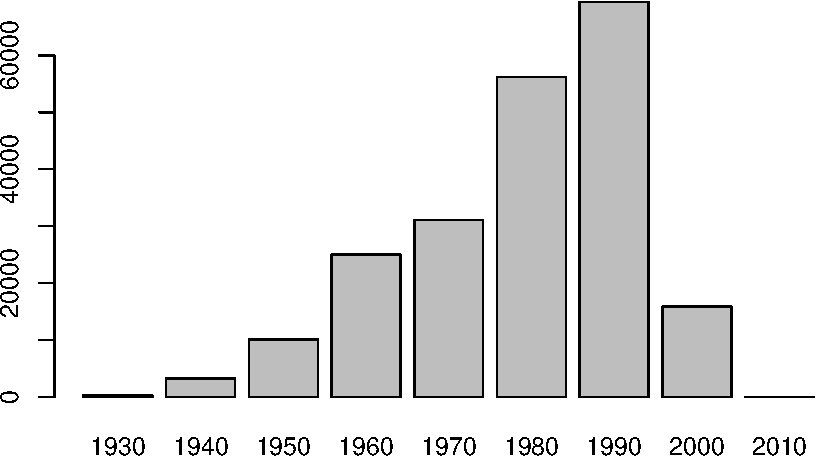
\includegraphics{R-data-wrangling_files/figure-latex/driver-birth-cohorts-1.pdf}
\caption{\label{fig:driver-birth-cohorts}Driver Birth Cohorts}
\end{figure}

Mutate can also be used in conjunction with logical conditions. For example, we could create a new column, where we assign everyone born after the year 2000 to a group ``millenial'' and overyone before to ``pre-millenial''.

In order to do this we take advantage of the \texttt{ifelse} function:

\texttt{ifelse(a\_logical\_condition,\ if\_true\_return\_this,\ if\_false\_return\_this)}

In conjunction with mutate, this works like this:

\begin{Shaded}
\begin{Highlighting}[]
\NormalTok{stops }\SpecialCharTok{\%\textgreater{}\%} 
  \FunctionTok{mutate}\NormalTok{(}\AttributeTok{cohort =} \FunctionTok{ifelse}\NormalTok{(}\FunctionTok{year}\NormalTok{(driver\_birthdate) }\SpecialCharTok{\textless{}} \DecValTok{2000}\NormalTok{, }\StringTok{"pre{-}millenial"}\NormalTok{, }\StringTok{"millenial"}\NormalTok{)) }\SpecialCharTok{\%\textgreater{}\%} 
  \FunctionTok{select}\NormalTok{(driver\_birthdate, cohort)}
\end{Highlighting}
\end{Shaded}

\begin{verbatim}
#> # A tibble: 211,211 x 2
#>    driver_birthdate cohort       
#>    <date>           <chr>        
#>  1 1950-06-14       pre-millenial
#>  2 1967-04-06       pre-millenial
#>  3 1974-04-15       pre-millenial
#>  4 1981-03-23       pre-millenial
#>  5 1992-08-03       pre-millenial
#>  6 1960-05-02       pre-millenial
#>  7 1953-03-16       pre-millenial
#>  8 1993-06-14       pre-millenial
#>  9 1947-12-11       pre-millenial
#> 10 1984-07-14       pre-millenial
#> # ... with 211,201 more rows
\end{verbatim}

More advanced conditional recoding can be done with \href{https://dplyr.tidyverse.org/reference/case_when.html}{\texttt{case\_when()}}.

\begin{quote}
Challenge

Create a new data frame from the \texttt{stops} data that meets the following
criteria: contains only the \texttt{violation} column for female drivers of age 50 that were stopped on a Sunday. For this add a new column to your data frame called
\texttt{weekday\_of\_stop} containing the number of the weekday when the stop occurred. Use the \texttt{wday()} function from \texttt{lubridate} (Sunday = 1).

Think about how the commands should be ordered to produce this data frame!
\end{quote}

\hypertarget{what-is-split-apply-combine}{%
\section{What is split-apply-combine?}\label{what-is-split-apply-combine}}

Many data analysis tasks can be approached using the \emph{split-apply-combine}
paradigm: split the data into groups, apply some analysis to each group, and
then combine the results.

\begin{figure}
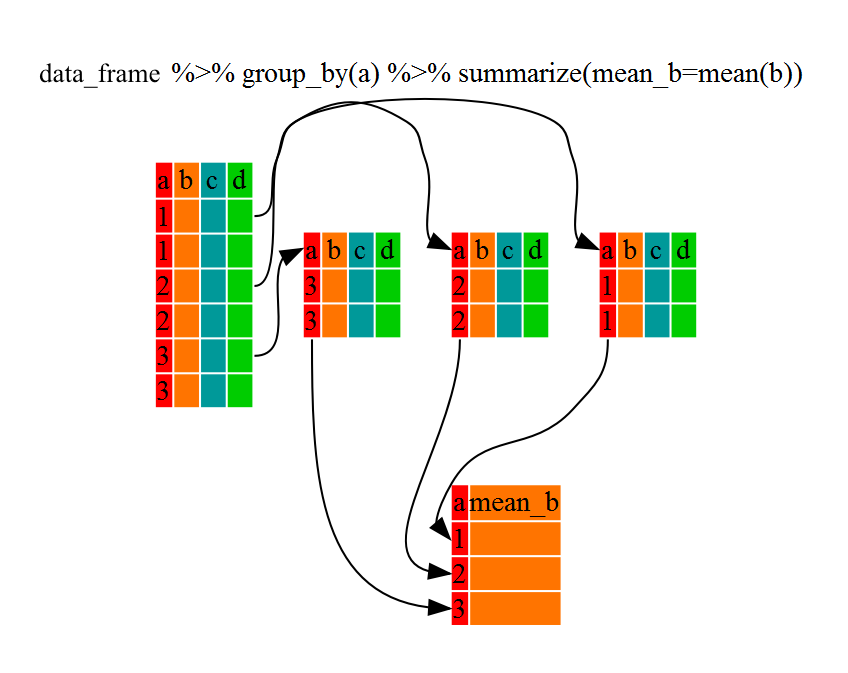
\includegraphics[width=\textwidth]{img/split-apply-combine} \caption{Split - Apply - Combine}\label{fig:split-apply-combine}
\end{figure}

\textbf{\texttt{dplyr}} makes this possible through the use of the \texttt{group\_by()} function.

\texttt{group\_by()} is often used together with \texttt{summarize()}, which collapses each
group into a single-row summary of that group. \texttt{group\_by()} takes as arguments
the column names that contain the \textbf{categorical} variables for which you want
to calculate the summary statistics. So to view the mean age for black and white drivers:

\begin{Shaded}
\begin{Highlighting}[]
\NormalTok{stops }\SpecialCharTok{\%\textgreater{}\%}
  \FunctionTok{group\_by}\NormalTok{(driver\_race) }\SpecialCharTok{\%\textgreater{}\%}
  \FunctionTok{summarize}\NormalTok{(}\AttributeTok{mean\_age =} \FunctionTok{mean}\NormalTok{(driver\_age, }\AttributeTok{na.rm=}\ConstantTok{TRUE}\NormalTok{))}
\end{Highlighting}
\end{Shaded}

\begin{verbatim}
#> `summarise()` ungrouping output (override with `.groups` argument)
\end{verbatim}

\begin{verbatim}
#> # A tibble: 3 x 2
#>   driver_race mean_age
#>   <chr>          <dbl>
#> 1 Black           34.2
#> 2 White           36.2
#> 3 <NA>            34.5
\end{verbatim}

If we wanted to remove the line with \texttt{NA} we could insert a \texttt{filter()} in the chain:

\begin{Shaded}
\begin{Highlighting}[]
\NormalTok{stops }\SpecialCharTok{\%\textgreater{}\%}
  \FunctionTok{filter}\NormalTok{(}\SpecialCharTok{!}\FunctionTok{is.na}\NormalTok{(driver\_race)) }\SpecialCharTok{\%\textgreater{}\%} 
  \FunctionTok{group\_by}\NormalTok{(driver\_race) }\SpecialCharTok{\%\textgreater{}\%}
  \FunctionTok{summarize}\NormalTok{(}\AttributeTok{mean\_age =} \FunctionTok{mean}\NormalTok{(driver\_age, }\AttributeTok{na.rm=}\ConstantTok{TRUE}\NormalTok{))}
\end{Highlighting}
\end{Shaded}

\begin{verbatim}
#> `summarise()` ungrouping output (override with `.groups` argument)
\end{verbatim}

\begin{verbatim}
#> # A tibble: 2 x 2
#>   driver_race mean_age
#>   <chr>          <dbl>
#> 1 Black           34.2
#> 2 White           36.2
\end{verbatim}

Recall that \texttt{is.na()} is a function that determines whether something is an \texttt{NA}. The \texttt{!} symbol negates the result, so we're asking for everything that is \emph{not} an \texttt{NA}.

You can also group by multiple columns:

\begin{Shaded}
\begin{Highlighting}[]
\NormalTok{stops }\SpecialCharTok{\%\textgreater{}\%} 
  \FunctionTok{filter}\NormalTok{(}\SpecialCharTok{!}\FunctionTok{is.na}\NormalTok{(driver\_race)) }\SpecialCharTok{\%\textgreater{}\%}
  \FunctionTok{group\_by}\NormalTok{(county\_name, driver\_race) }\SpecialCharTok{\%\textgreater{}\%}
  \FunctionTok{summarize}\NormalTok{(}\AttributeTok{mean\_age =} \FunctionTok{mean}\NormalTok{(driver\_age, }\AttributeTok{na.rm=}\ConstantTok{TRUE}\NormalTok{))}
\end{Highlighting}
\end{Shaded}

\begin{verbatim}
#> `summarise()` regrouping output by 'county_name' (override with `.groups` argument)
\end{verbatim}

\begin{verbatim}
#> # A tibble: 163 x 3
#> # Groups:   county_name [82]
#>    county_name driver_race mean_age
#>    <chr>       <chr>          <dbl>
#>  1 Adams       Black           36.2
#>  2 Adams       White           40.0
#>  3 Alcorn      Black           34.6
#>  4 Alcorn      White           33.6
#>  5 Amite       Black           37.5
#>  6 Amite       White           42.1
#>  7 Attala      Black           36.4
#>  8 Attala      White           38.6
#>  9 Benton      Black           34.7
#> 10 Benton      White           32.0
#> # ... with 153 more rows
\end{verbatim}

Once the data are grouped, you can also summarize multiple variables at the same
time (and not necessarily on the same variable). For instance, we could add a
column indicating the minimum age in each group (i.e.~county):

\begin{Shaded}
\begin{Highlighting}[]
\NormalTok{stops }\SpecialCharTok{\%\textgreater{}\%}
  \FunctionTok{filter}\NormalTok{(}\SpecialCharTok{!}\FunctionTok{is.na}\NormalTok{(driver\_race)) }\SpecialCharTok{\%\textgreater{}\%} 
  \FunctionTok{group\_by}\NormalTok{(county\_name, driver\_race) }\SpecialCharTok{\%\textgreater{}\%}
  \FunctionTok{summarize}\NormalTok{(}\AttributeTok{mean\_age =} \FunctionTok{mean}\NormalTok{(driver\_age, }\AttributeTok{na.rm=}\ConstantTok{TRUE}\NormalTok{),}
            \AttributeTok{min\_age =} \FunctionTok{min}\NormalTok{(driver\_age, }\AttributeTok{na.rm=}\ConstantTok{TRUE}\NormalTok{))}
\end{Highlighting}
\end{Shaded}

\begin{verbatim}
#> `summarise()` regrouping output by 'county_name' (override with `.groups` argument)
\end{verbatim}

\begin{verbatim}
#> # A tibble: 163 x 4
#> # Groups:   county_name [82]
#>    county_name driver_race mean_age min_age
#>    <chr>       <chr>          <dbl>   <dbl>
#>  1 Adams       Black           36.2      16
#>  2 Adams       White           40.0      16
#>  3 Alcorn      Black           34.6      17
#>  4 Alcorn      White           33.6      15
#>  5 Amite       Black           37.5      17
#>  6 Amite       White           42.1      15
#>  7 Attala      Black           36.4       8
#>  8 Attala      White           38.6      15
#>  9 Benton      Black           34.7      18
#> 10 Benton      White           32.0      18
#> # ... with 153 more rows
\end{verbatim}

\hypertarget{tallying}{%
\section{Tallying}\label{tallying}}

When working with data, it is also common to want to know the number of
observations found for categorical variables. For this, \textbf{\texttt{dplyr}}
provides \texttt{count()}. For example, if we wanted to see how many traffic stops each officer recorded:

\begin{Shaded}
\begin{Highlighting}[]
\NormalTok{stops }\SpecialCharTok{\%\textgreater{}\%}
  \FunctionTok{count}\NormalTok{(officer\_id)}
\end{Highlighting}
\end{Shaded}

Bu default, count will name the column with the counts \texttt{n}. We can change this by explicitly providing a value for the \texttt{name} argument:

\begin{Shaded}
\begin{Highlighting}[]
\NormalTok{stops }\SpecialCharTok{\%\textgreater{}\%}
  \FunctionTok{count}\NormalTok{(officer\_id, }\AttributeTok{name =} \StringTok{"n\_stops"}\NormalTok{)}
\end{Highlighting}
\end{Shaded}

We can optionally sort the results in descending order by adding \texttt{sort=TRUE}:

\begin{Shaded}
\begin{Highlighting}[]
\NormalTok{stops }\SpecialCharTok{\%\textgreater{}\%}
  \FunctionTok{count}\NormalTok{(officer\_id, }\AttributeTok{name =} \StringTok{"n\_stops"}\NormalTok{, }\AttributeTok{sort =} \ConstantTok{TRUE}\NormalTok{)}
\end{Highlighting}
\end{Shaded}

\texttt{count()} calls \texttt{group\_by()} transparently before counting the total number of records for each category. Similarly, we can count subgroups within groups:

\begin{Shaded}
\begin{Highlighting}[]
\NormalTok{stops }\SpecialCharTok{\%\textgreater{}\%}
  \FunctionTok{count}\NormalTok{(officer\_id, violation, }\AttributeTok{name =} \StringTok{"n\_stops"}\NormalTok{)}
\end{Highlighting}
\end{Shaded}

Alternatives:

\begin{Shaded}
\begin{Highlighting}[]
\NormalTok{stops }\SpecialCharTok{\%\textgreater{}\%}
  \FunctionTok{group\_by}\NormalTok{(officer\_id) }\SpecialCharTok{\%\textgreater{}\%} 
  \FunctionTok{tally}\NormalTok{(}\AttributeTok{sort =} \ConstantTok{TRUE}\NormalTok{) }\CommentTok{\# tally() requires group\_by before counting}

\NormalTok{stops }\SpecialCharTok{\%\textgreater{}\%}
  \FunctionTok{group\_by}\NormalTok{(officer\_id) }\SpecialCharTok{\%\textgreater{}\%}
  \FunctionTok{summarize}\NormalTok{(}\AttributeTok{n =} \FunctionTok{n}\NormalTok{()) }\SpecialCharTok{\%\textgreater{}\%} \CommentTok{\# n() is useful when the count is needed within a calculation}
  \FunctionTok{arrange}\NormalTok{(}\FunctionTok{desc}\NormalTok{(n))}
\end{Highlighting}
\end{Shaded}

\begin{quote}
Challenge

Which 5 counties were the ones with the most stops in 2013?
Hint: use the year() function from lubridate.
\end{quote}

\hypertarget{joining-two-tables}{%
\section{Joining two tables}\label{joining-two-tables}}

It is not uncommon that we have our data spread out in different tables and need to bring those together for analysis. In this example we will combine the numbers of stops for black and white drivers per county together with the numbers of the black and white total population for these counties. The population data are the estimated values of the 5 year average from the 2011-2015 American Community Survey (ACS):

\begin{Shaded}
\begin{Highlighting}[]
\NormalTok{acs }\OtherTok{\textless{}{-}} \FunctionTok{read\_csv}\NormalTok{(}\StringTok{"data/MS\_acs2015\_bw.csv"}\NormalTok{)}
\end{Highlighting}
\end{Shaded}

\begin{verbatim}
#> Parsed with column specification:
#> cols(
#>   County = col_character(),
#>   FIPS = col_double(),
#>   black_pop = col_double(),
#>   white_pop = col_double(),
#>   bw_pop = col_double()
#> )
\end{verbatim}

\begin{Shaded}
\begin{Highlighting}[]
\NormalTok{acs}
\end{Highlighting}
\end{Shaded}

\begin{verbatim}
#> # A tibble: 82 x 5
#>    County      FIPS black_pop white_pop bw_pop
#>    <chr>      <dbl>     <dbl>     <dbl>  <dbl>
#>  1 Jones      28067     19711     47154  66865
#>  2 Lauderdale 28075     33893     43482  77375
#>  3 Pike       28113     21028     18282  39310
#>  4 Hancock    28045      4172     39686  43858
#>  5 Holmes     28051     15498      3105  18603
#>  6 Jackson    28059     30704    101686 132390
#>  7 Grenada    28043      9417     11991  21408
#>  8 Scott      28123     10562     16920  27482
#>  9 Wayne      28153      8015     12154  20169
#> 10 Bolivar    28011     21648     11197  32845
#> # ... with 72 more rows
\end{verbatim}

In a first step we count all the stops per county.

\begin{Shaded}
\begin{Highlighting}[]
\NormalTok{stops }\SpecialCharTok{\%\textgreater{}\%} 
  \FunctionTok{count}\NormalTok{(county\_name, }\AttributeTok{name =} \StringTok{"n\_stops"}\NormalTok{) }
\end{Highlighting}
\end{Shaded}

\begin{verbatim}
#> # A tibble: 82 x 2
#>    county_name n_stops
#>    <chr>         <int>
#>  1 Adams           942
#>  2 Alcorn         3345
#>  3 Amite          2921
#>  4 Attala         4203
#>  5 Benton          214
#>  6 Bolivar        4526
#>  7 Calhoun        1658
#>  8 Carroll        1788
#>  9 Chickasaw      3869
#> 10 Choctaw         613
#> # ... with 72 more rows
\end{verbatim}

We will then pipe this into our next operation where we bring the two tables together. We will use \texttt{left\_join}, which returns all rows from the left table, and all columns from the left and the right table. As ID, which uniquely identifies the corresponding records in each table we use the County names.

\begin{Shaded}
\begin{Highlighting}[]
\NormalTok{stops }\SpecialCharTok{\%\textgreater{}\%} 
  \FunctionTok{count}\NormalTok{(county\_name, }\AttributeTok{name =} \StringTok{"n\_stops"}\NormalTok{) }\SpecialCharTok{\%\textgreater{}\%} 
  \FunctionTok{left\_join}\NormalTok{(acs, }\AttributeTok{by =} \FunctionTok{c}\NormalTok{(}\StringTok{"county\_name"} \OtherTok{=} \StringTok{"County"}\NormalTok{)) }
\end{Highlighting}
\end{Shaded}

\begin{verbatim}
#> # A tibble: 82 x 6
#>    county_name n_stops  FIPS black_pop white_pop bw_pop
#>    <chr>         <int> <dbl>     <dbl>     <dbl>  <dbl>
#>  1 Adams           942 28001     17757     12856  30613
#>  2 Alcorn         3345 28003      4281     31563  35844
#>  3 Amite          2921 28005      5416      7395  12811
#>  4 Attala         4203 28007      8194     10649  18843
#>  5 Benton          214 28009      3078      5166   8244
#>  6 Bolivar        4526 28011     21648     11197  32845
#>  7 Calhoun        1658 28013      3991     10103  14094
#>  8 Carroll        1788 28015      3470      6702  10172
#>  9 Chickasaw      3869 28017      7549      9522  17071
#> 10 Choctaw         613 28019      2596      5661   8257
#> # ... with 72 more rows
\end{verbatim}

Now we can, for example calculate the stop rate, i.e.~the number of stops per population in each county.

\begin{quote}
Challenge

Which county has the highest and which one the lowest stop rate?
Use the snippet from above and pipe into the additional operations
to do this.
\end{quote}

\texttt{dplyr} join functions are generally equivalent to \texttt{merge} from the base command, but there are a few advantages:

\begin{itemize}
\tightlist
\item
  rows are kept in existing order
\item
  it runs faster
\item
  tells you what keys you're merging by (if you don't supply them)
\item
  also works with database tables.
\end{itemize}

\url{https://groups.google.com/d/msg/manipulatr/OuAPC4VyfIc/Qnt8mDfq0WwJ}

See \texttt{?dplyr::join} for all the possible joins.

\hypertarget{tidyr}{%
\chapter{\texorpdfstring{Data Manipulation using \textbf{\texttt{tidyr}}}{Data Manipulation using tidyr}}\label{tidyr}}

\begin{quote}
Learning Objectives

\begin{itemize}
\tightlist
\item
  Understand the concept of a wide and a long table format and for which purpose those formats are useful.
\item
  Understand what key-value pairs are.
\item
  Reshape a data frame from long to wide format and back with the \texttt{pivot\_wider} and \texttt{pivot\_longer} commands from the \textbf{\texttt{tidyr}} package.
\item
  Export a data frame to a .csv file.
\end{itemize}
\end{quote}

\begin{center}\rule{0.5\linewidth}{0.5pt}\end{center}

\texttt{dplyr} pairs nicely with \textbf{\texttt{tidyr}} which enables you to swiftly convert between different data formats for plotting and analysis.

The package \textbf{\texttt{tidyr}} addresses the common problem of wanting to reshape your data for plotting and use by different R functions. Sometimes we want data sets where we have one row per observation. Sometimes we want a data frame where each observation type has its own column, and rows are instead more aggregated groups - like surveys, where each column represents an answer. Moving back and forth between these formats is nontrivial, and \textbf{\texttt{tidyr}} gives you tools for this and more sophisticated data manipulation.

To learn more about \textbf{\texttt{tidyr}} after the workshop, you may want to check out this \href{https://github.com/rstudio/cheatsheets/raw/master/data-import.pdf}{cheatsheet about \textbf{\texttt{tidyr}}}.

\hypertarget{about-long-and-wide-table-format}{%
\section{About long and wide table format}\label{about-long-and-wide-table-format}}

The `long' format is where:

\begin{itemize}
\tightlist
\item
  each column is a variable
\item
  each row is an observation
\end{itemize}

In the `long' format, you usually have 1 column for the observed variable and
the other columns are ID variables.

For the `wide' format a row, for example could be a reserarch subject for which you have multiple observation variables containing the same type of data, for example responses to a set of survey questions, or repeated observations over time, or a mix of both. Here is an example:

\begin{table}[ht]
\centering
\begin{tabular}{rlrrr}
  \hline
 & subject\_ID & question\_1 & question\_2 & question\_3 \\ 
  \hline
1 & A & 4.00 & 3.00 & 4.00 \\ 
  2 & B & 4.00 & 1.00 & 5.00 \\ 
  3 & C & 2.00 & 5.00 & 2.00 \\ 
   \hline
\end{tabular}
\end{table}

You may find data input may be simpler or some other
applications may prefer the `wide' format. However, many of \texttt{R}`s functions have
been designed assuming you have 'long' format data. This tutorial will help you
efficiently transform your data regardless of original format.

\begin{figure}
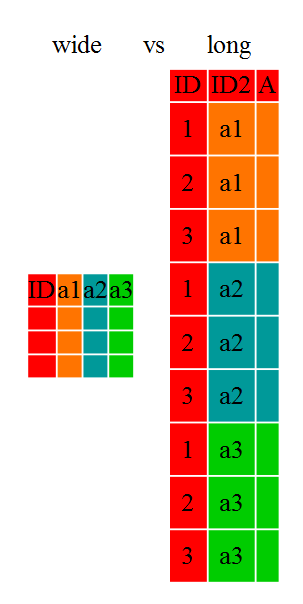
\includegraphics[width=0.3\linewidth]{img/wide-vs-long} \caption{Wide vs. Long Table Format}\label{fig:wide-vs-long}
\end{figure}

The choice of data format affects readability. For humans, the wide format is often more intuitive, since we can often see more of the data on the screen due to its shape. However, the long format is more machine readable and is closer to the formatting of databases. The \texttt{ID} variables in our dataframes are similar to the fields in a database and observed variables are like the database values.

\begin{quote}
Challenge 1

Is stops in a long or wide format?
\end{quote}

\hypertarget{long-to-wide-with-pivot_wider}{%
\section{\texorpdfstring{Long to Wide with \texttt{pivot\_wider}}{Long to Wide with pivot\_wider}}\label{long-to-wide-with-pivot_wider}}

Now let's see this in action. First, using \textbf{\texttt{dplyr}}, let's create a data frame with the counts of different violations for each county:

\begin{Shaded}
\begin{Highlighting}[]
\NormalTok{violations }\OtherTok{\textless{}{-}}\NormalTok{ stops }\SpecialCharTok{\%\textgreater{}\%}
  \FunctionTok{count}\NormalTok{(county\_name, violation)}

\NormalTok{violations}
\end{Highlighting}
\end{Shaded}

\begin{verbatim}
#>   county_name                violation   n
#> 1       Adams        Breaks-Lights-etc   7
#> 2       Adams         Careless driving  48
#> 3       Adams License-Permit-Insurance 118
#> 4       Adams         Other or unknown  35
#> 5       Adams                Seat belt 229
#> 6       Adams                 Speeding 505
\end{verbatim}

Now, to make this long data wide, we use \texttt{pivot\_wider} from \texttt{tidyr} to turn the driver gender into columns. In addition to our data table we provide \texttt{pivot\_wider} with two arguments: \texttt{names\_from} describes which column to use for name of the output column, and \texttt{values\_from} tells it from column to get the cell values. We'll use a pipe so we can ignore the data argument.

\begin{Shaded}
\begin{Highlighting}[]
\NormalTok{violations\_wide }\OtherTok{\textless{}{-}}\NormalTok{ violations }\SpecialCharTok{\%\textgreater{}\%}
  \FunctionTok{pivot\_wider}\NormalTok{(}\AttributeTok{names\_from =}\NormalTok{ violation, }
              \AttributeTok{values\_from =}\NormalTok{ n) }

\NormalTok{violations\_wide}
\end{Highlighting}
\end{Shaded}

\begin{verbatim}
#> # A tibble: 82 x 7
#>    county_name `Breaks-Lights-~ `Careless drivi~ `License-Permit~
#>    <chr>                  <int>            <int>            <int>
#>  1 Adams                      7               48              118
#>  2 Alcorn                    62              100              737
#>  3 Amite                     47               86              370
#>  4 Attala                    99              113              526
#>  5 Benton                     3                9               73
#>  6 Bolivar                   57              139             1034
#>  7 Calhoun                   26               38              383
#>  8 Carroll                   26               40              323
#>  9 Chickasaw                 42               53             1378
#> 10 Choctaw                    8                6               73
#> # ... with 72 more rows, and 3 more variables: `Other or unknown` <int>, `Seat
#> #   belt` <int>, Speeding <int>
\end{verbatim}

\hypertarget{wide-to-long-with-pivot_longer}{%
\section{\texorpdfstring{Wide to long with \texttt{pivot\_longer}}{Wide to long with pivot\_longer}}\label{wide-to-long-with-pivot_longer}}

What if we had the opposite problem, and wanted to go from a wide to long
format? For that, we use \texttt{pivot\_longer}, which will increase the number of rows and decrease the number of columns. We provide the functino with thee arguments: \texttt{cols} which are the columns we want to pivot into the long format, \texttt{names\_to}, which is a string specifying the name of the column to create from the data stored in the column names, and \texttt{values\_to}, which is also a string, specifying the name of the column to create from the data stored in cell values.
So, to go backwards from \texttt{violations\_wide}, and exclude \texttt{county\_name} from the long format, we would do the following:

\begin{Shaded}
\begin{Highlighting}[]
\NormalTok{violations\_long }\OtherTok{\textless{}{-}}\NormalTok{ violations\_wide }\SpecialCharTok{\%\textgreater{}\%}
  \FunctionTok{pivot\_longer}\NormalTok{(}\AttributeTok{cols =} \SpecialCharTok{{-}}\NormalTok{county\_name,        }\CommentTok{\# exclude column with county name}
               \AttributeTok{names\_to =} \StringTok{"violation"}\NormalTok{,     }\CommentTok{\# name is a string!}
               \AttributeTok{values\_to =} \StringTok{"n"}\NormalTok{)            }\CommentTok{\# also a string}

\NormalTok{violations\_long}
\end{Highlighting}
\end{Shaded}

\begin{verbatim}
#> # A tibble: 492 x 3
#>    county_name violation                    n
#>    <chr>       <chr>                    <int>
#>  1 Adams       Breaks-Lights-etc            7
#>  2 Adams       Careless driving            48
#>  3 Adams       License-Permit-Insurance   118
#>  4 Adams       Other or unknown            35
#>  5 Adams       Seat belt                  229
#>  6 Adams       Speeding                   505
#>  7 Alcorn      Breaks-Lights-etc           62
#>  8 Alcorn      Careless driving           100
#>  9 Alcorn      License-Permit-Insurance   737
#> 10 Alcorn      Other or unknown           418
#> # ... with 482 more rows
\end{verbatim}

We could also have used a specification for what columns to include. This can be
useful if you have a large number of identifying columns, and it's easier to
specify what to gather than what to leave alone. And if the columns are adjacent to each other, we don't even need to list them all out -- we can use the \texttt{:} operator!

\begin{Shaded}
\begin{Highlighting}[]
\NormalTok{violations\_wide }\SpecialCharTok{\%\textgreater{}\%}
  \FunctionTok{pivot\_longer}\NormalTok{(}\AttributeTok{cols =} \StringTok{\textasciigrave{}}\AttributeTok{Breaks{-}Lights{-}etc}\StringTok{\textasciigrave{}}\SpecialCharTok{:}\NormalTok{Speeding,      }\CommentTok{\# this also works}
               \AttributeTok{names\_to =} \StringTok{"violation"}\NormalTok{, }
               \AttributeTok{values\_to =} \StringTok{"n"}\NormalTok{)}
\end{Highlighting}
\end{Shaded}

\begin{verbatim}
#> # A tibble: 492 x 3
#>    county_name violation                    n
#>    <chr>       <chr>                    <int>
#>  1 Adams       Breaks-Lights-etc            7
#>  2 Adams       Careless driving            48
#>  3 Adams       License-Permit-Insurance   118
#>  4 Adams       Other or unknown            35
#>  5 Adams       Seat belt                  229
#>  6 Adams       Speeding                   505
#>  7 Alcorn      Breaks-Lights-etc           62
#>  8 Alcorn      Careless driving           100
#>  9 Alcorn      License-Permit-Insurance   737
#> 10 Alcorn      Other or unknown           418
#> # ... with 482 more rows
\end{verbatim}

There are many powerful operations you can do with the \texttt{pivot\_*} functions. To learn more review the vignette:

\begin{Shaded}
\begin{Highlighting}[]
\FunctionTok{vignette}\NormalTok{(}\StringTok{"pivot"}\NormalTok{)}
\end{Highlighting}
\end{Shaded}

\begin{quote}
Challenge

1.From the stops dataframe create a wide data frame \texttt{tr\_wide} with
``year'' as columns, each row is a different violation,
and the values are the
number of traffic stops per each violation, roughly like this:

\texttt{violation\ \ \ \ \ \ \textbar{}\ 2013\ \textbar{}\ 2014\ \textbar{}\ 2015\ ...}
\texttt{Break-Lights\ \ \ \textbar{}\ \ \ 65\ \textbar{}\ \ \ \ 54\textbar{}\ \ \ 67\ ...}
\texttt{Speeding\ \ \ \ \ \ \ \textbar{}\ \ 713\ \textbar{}\ \ \ 948\textbar{}\ \ 978\ ...}
\texttt{...}

Use \texttt{year()} from the lubridate package. Hint: You will need to summarize
and count the traffic stops before reshaping the table.
\end{quote}

\begin{quote}
\begin{enumerate}
\def\labelenumi{\arabic{enumi}.}
\setcounter{enumi}{1}
\tightlist
\item
  Now take the data frame, and make it long again, so each row is a
  unique violation - year combination, like this:
\end{enumerate}

\texttt{violation\ \ \textbar{}\ year\ \textbar{}\ n\ of\ stops}
\texttt{Speeding\ \ \ \textbar{}\ 2013\ \textbar{}\ 65}
\texttt{Speeding\ \ \ \textbar{}\ 2014\ \textbar{}\ 54}
\texttt{...\ etc}
\end{quote}

\hypertarget{exporting-data}{%
\section{Exporting data}\label{exporting-data}}

Similar to the \texttt{read\_csv()} function used for reading CSV files into R, there is a \texttt{write\_csv()} function that generates CSV files from data frames.

Before using \texttt{write\_csv()}, we are going to create a new folder, \texttt{data\_output},
in our working directory that will store this generated dataset. We don't want
to write generated datasets in the same directory as our raw data. It's good
practice to keep them separate. The \texttt{data} folder should only contain the raw,
unaltered data, and should be left alone to make sure we don't delete or modify
it. In contrast, our script will generate the contents of the \texttt{data\_output}
directory, so even if the files it contains are deleted, we can always
re-generate them.

We can now save the table generated above in our \texttt{data\_output}
folder:

\begin{Shaded}
\begin{Highlighting}[]
\FunctionTok{write\_csv}\NormalTok{(violation\_wide, }\StringTok{"data\_output/county\_violations.csv"}\NormalTok{)}
\end{Highlighting}
\end{Shaded}


  \bibliography{book.bib,packages.bib}

\end{document}
